\chapter{Species and forms}
\label{chap:species}
Pokémon are partitioned into species.
Each species is identified by its own Pokédex number.
As we will see, this number is the only thing guaranteed to be shared
 among all the population of a species.

\section{Forms}
\label{sec:forms}
Some species boast multiple forms and genders, all sharing one common Pokédex entry.
Form is usually merely a visual distinction, but it is sometimes reflected
 in stats or even typing.
All Pokémon of a given form share the same Attack (ATK), Defense (DEF), and
 Stamina (STA) base statistics.
These statistics are always positive integers.

Common forms include \textit{Mega}, a temporary form with greater ATK and DEF (see \autoref{sec:mega}),
  \textit{Dynamax} and \textit{Gigantamax}, temporary forms with the ability to use
  powerful attacks (see \autoref{sec:dmax} and \autoref{sec:gmax}),
  and \textit{Shiny}, a visually distinctive and rare form (see \autoref{sec:shiny}).
Regional forms are also seen: Alolan, Galarian, Hisuian, and Paldean.
Gender, if differentiated at all, is usually a small change to
 appearance or call, but it (like other forms) also affects a few evolutionary
 paths.

\section{Evolution}
\label{sec:evolution}
Some species can, under the correct conditions, evolve into others.
We call the set of Pokémon related by evolution operations a genus.
Change of form is not an evolution, since the species remains the same.
We call a Pokémon that has undergone $N$ evolutions a Stage $N+1$ Pokémon.
No Pokémon of Stage 4 or higher currently exist.
Evolution (unlike some form changes) is irreversible.
Evolution does not necessarily preserve typing, i.e.\ typing is not always
  constant within a genus (\autoref{table:heteroevolve})\footnote{It is interesting
  that Sharpedo changes from Water+Dark to Mega Sharpedo's Dark+Water,
  a functionally equivalent typing. When this kind of thing happens,
  I assume it due to conformance with other Pokémon games, but never
  rule out simple fuckups.}.
\input{out/hetero}
Almost all evolutions require that Candy of that genus (Zygarde is an exception),
  and some evolutions depend upon some condition (\autoref{table:condevolutions})
  or catalyzing item, which is consumed (\autoref{table:itemevolutions})
Evolution generally improves base stats \textbf{(FIXME: are there exceptions?)},
  and typically makes available new, more powerful attacks.
Evolution revives a Pokémon if it is fainted, and always fully restores HP\@.

\begin{table}[ht]
\footnotesize
\begin{center}
  \begin{tabular}{lll}
    Base & Requirements & Result \\
    \Midrule
  \end{tabular}
\end{center}
\caption{Evolutions dependent upon a condition}
\label{table:condevolutions}
\end{table}

\begin{table}[ht]
\footnotesize
\begin{center}
  \begin{tabular}{lll}
    Base & Requirements & Result \\
    \Midrule
    Gloom & 100 Oddish candy + 
\includegraphics[width=1em,height=1em]{images/sunstone.png} & Bellossom \\
    Sunkern & 50 Sunkern candy + 
\includegraphics[width=1em,height=1em]{images/sunstone.png} & Sunflora \\
    Cottonee & 50 Cottonee candy + 
\includegraphics[width=1em,height=1em]{images/sunstone.png} & Whimsicott \\
    Petilil & 50 Petilil candy + 
\includegraphics[width=1em,height=1em]{images/sunstone.png} & Lilligant \\
    Helioptile & 50 Helioptile candy + 
\includegraphics[width=1em,height=1em]{images/sunstone.png} & Heliolisk \\
    Poliwhirl & 100 Poliwag candy + 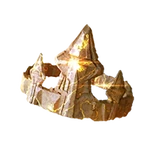
\includegraphics[width=1em,height=1em]{images/kingsrock.png} & Politoed \\
    Slowpoke & 50 Slowpoke candy + 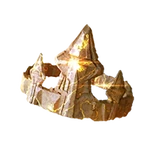
\includegraphics[width=1em,height=1em]{images/kingsrock.png} & Slowking \\
    Onix & 50 Onix candy + 
\includegraphics[width=1em,height=1em]{images/metalcoat.png} & Steelix \\
    Scyther & 50 Scyther candy + 
\includegraphics[width=1em,height=1em]{images/metalcoat.png} & Scizor \\
    Seadra & 100 Horsea candy + 
\includegraphics[width=1em,height=1em]{images/dragonscale.png} & Kingdra \\
    Porygon & 25 Porygon candy + 
\includegraphics[width=1em,height=1em]{images/upgrade.png} & Porygon2 \\
    Poygon2 & 100 Porygon candy + 
\includegraphics[width=1em,height=1em]{images/sinnohstone.png} & Porygon-Z \\
    Lickitung & 100 Lickitung Candy + 
\includegraphics[width=1em,height=1em]{images/sinnohstone.png} & Lickilicky \\
    Tangela	& 100 Tangela Candy + 
\includegraphics[width=1em,height=1em]{images/sinnohstone.png} & Tangrowth \\
    Electabuzz & 100 Elekid Candy + 
\includegraphics[width=1em,height=1em]{images/sinnohstone.png} & Electivire	\\
    Magmar & 100 Magby Candy + 
\includegraphics[width=1em,height=1em]{images/sinnohstone.png} & Magmortar	\\
    Sneasel & 100 Sneasel Candy + 
\includegraphics[width=1em,height=1em]{images/sinnohstone.png} & Weavile	\\
    Togetic & 100 Togepi Candy + 
\includegraphics[width=1em,height=1em]{images/sinnohstone.png} & Togekiss	\\
    Yanma & 100 Yanma Candy + 
\includegraphics[width=1em,height=1em]{images/sinnohstone.png} & Yanmega	\\
    Gligar & 100 Gligar Candy + 
\includegraphics[width=1em,height=1em]{images/sinnohstone.png} & Gliscor	\\
    Murkrow & 100 Murkrow Candy + 
\includegraphics[width=1em,height=1em]{images/sinnohstone.png} & Honchkrow	\\
    Male Kirlia & 100 Ralts Candy + 
\includegraphics[width=1em,height=1em]{images/sinnohstone.png} & Gallade	\\
    Misdreavus & 100 Misdreavus Candy + 
\includegraphics[width=1em,height=1em]{images/sinnohstone.png} & Mismagius	\\
    Piloswine & 100 Swinub Candy + 
\includegraphics[width=1em,height=1em]{images/sinnohstone.png} & Mamoswine	\\
    Dusclops & 100 Duskull Candy + 
\includegraphics[width=1em,height=1em]{images/sinnohstone.png} & Dusknoir	\\
    Female Snorunt & 100 Snorunt Candy + 
\includegraphics[width=1em,height=1em]{images/sinnohstone.png} & Froslass	\\
    Aipom & 100 Aipom Candy + 
\includegraphics[width=1em,height=1em]{images/sinnohstone.png} & Ambipom	\\
    Roselia & 100 Budew Candy + 
\includegraphics[width=1em,height=1em]{images/sinnohstone.png} & Roserade	\\
    Applin & 200 Applin Candy + 20 
\includegraphics[width=1em,height=1em]{images/tartapple.png} & Flapple \\
    Applin & 200 Applin Candy + 20 
\includegraphics[width=1em,height=1em]{images/sweetapple.png} & Appletun \\
    Zygarde 10\% & 50 Zygarde Cubes & Zygarde 50\% \\
    Zygarde 50\% & 200 Zygarde Cubes & Zygarde Complete \\
  \end{tabular}
\end{center}
\caption{Evolutions dependent upon items}
\label{table:itemevolutions}
\end{table}

\subsection{Eevolution}
\begin{figure}
\end{figure}
Evolution within the Eevee genus is a complicated and unique affair.
Eevee (the species) can evolve into eight different species.
Five of these targets require some condition, and are deterministic.
If none of the conditions are met, the evolution is nondeterministic,
  with three possible results.
A second mechanism exists based on nicknames, deterministic across all eight targets,
  but it can only be used once per target per Trainer.
\textbf{FIXME: how do the two affect one another, which has priority?}
If the evolution is deterministic, the ``Evolve'' button will show the
  unique target.
It will otherwise show a question mark.
\textbf{FIXME: screenshot(s)}
Eevee's evolutions are often strong Pokémon early in the game.

For the nickname-based mechanic, give the Eevee you wish to evolve the nickname
  specified for the desired target from \autoref{table:eevee}.
\begin{table}
  \begin{center}
    \begin{tabular}{lrp{.5\textwidth}}
      Target & Nickname & Condition\\
      \Midrule
      Vaporeon & Rainer & Random\\
      Jolteon & Sparky & Random\\
      Flareon & Pyro & Random\\
      Sylveon & Kira & Earn 70 buddy hearts \\
      Espeon & Sakura & Walk 10 km with it as buddy,\newline Evolve during the day\\
      Umbreon & Tamao & Walk 10 km with it as buddy,\newline Evolve during the night\\
      Leafeon & Linnea & Evolve near an active Mossy Lure\\
      Glacion & Rea & Evolve near an active Glacial Lure\\
    \end{tabular}
  \end{center}
  \caption{Eevolution}
  \label{table:eevee}
\end{table}

\section{Shadow and Purified Pokémon}
\label{sec:shadow}
Team Rocket uses ``Shadow'' Pokémon modified for more attack
 and less defense capability than their base forms (for more details,
 see \autoref{sec:damage}).
Shadow Pokémon cost 20\% more than normal to evolve, teach second charged attacks, or power up.
When captured from Team Rocket, they enter their own Shadow Pokédex.
Captured Shadow Pokémon always know the charged attack Frustration.
Only during certain special events can this charged attack be replaced,
 at which time a Charged TM is required as normal.
It's a pretty terrible Charged Attack, and this really degrades the
 Shadow Pokémon until it can be replaced.
A Shadow Pokémon can be taught a second Charged Attack at any time.
Frustration is preserved across evolution, as is Shadow status itself.
Shadow Pokémon cannot be traded.

Purification of a Shadow Pokémon has a cost in Stardust and Candy.
Purified Pokémon cost 10\% less than normal to evolve, teach second charged attacks, or power up.
Purification enters the Pokémon into its own Purified Pokédex,
 advances it to level 25 if not yet there,
 eliminates the attack bonus and defense penalty,
 replaces the primary charged attack with Return (exclusive to purified Pokémon),
 and increases each IV component by 2  (up to the usual max of 15).
Return is preserved across evolution, as is Purified status itself.
Purified Pokémon can be traded, but constitute a Special Trade (\autoref{sec:trades}).

\section{Regions}
\label{sec:regions}
Each Pokémon is associated with one of eleven regions.
The region can be determined by their Pokédex index (\autoref{table:regions}).
\begin{table}[ht]
  \begin{center}
    \begin{tabular}{lrr}
      Region & Start & End\\
      \Midrule
      Kanto & \#0001 & \#0151\\
      Johto & \#0152 & \#0251\\
      Hoenn & \#0252 & \#0386\\
      Sinnoh & \#0387 & \#0493\\
      Unova & \#0494 & \#0649\\
      Kalos & \#0650 & \#0721\\
      Alola & \#0722 & \#0807\\
      Unknown & \#0808 & \#0809\\
      Galar & \#0810 & \#0898\\
      Hisui & \#0899 & \#0905\\
      Paldea & \#0906 & \#1025\\
    \end{tabular}
  \end{center}
  \caption{The regions of the Pokémon world (\textjapanese{ポケモンの世界})}
  \label{table:regions}
\end{table}

\section{Myths, Legends, and Beasts}
\label{sec:myths}
Legendary (\textjapanese{伝説のポケモン}) and Mythical (\textjapanese{幻のポケモン}) Pokémon
 are not generally seen in the wild.
They are members of the Pokémon mythos, heralds from times past and partly forgotten.
Some are so rare that their existence is doubted.
Ultra Beasts (\textjapanese{ウルトラビースト}) literally assault our dimension from
  another via ``Ultra Wormholes''.
Such Pokémon never hatch from eggs (\autoref{sec:eggs}), and are not usually included in wild spawn groups (\autoref{sec:spawns}).
They are instead typically Research rewards, or captured in raids.
It is not usually possible to accumulate more than one or two examples of Mythical
  Pokémon\footnote{Marshadow, Celebi, Mew, Shaymin, Victini, Meloetta, Keldeo,
  Jirachi, Diancie, Zarude, Zygarde, and Volcanion.}, making them prime
  candidates for Bottle Caps.
All have 20 km walk distances and cost 100,000 for second charged attacks.
They cannot be left in gyms (\autoref{sec:gyms}).

\section{Trends among species}
One thing to take away from \autoref{table:populations} is that the largest
  typings by population are the monotypes, representing 485 forms.
A majority of Pokédex have dual typing, but their diversity of typing means few dual types have much of a population.
Only Ground+Water, Flying+Normal, Bug+Poison, Grass+Ghost, Grass+Poison, Rock+Water, and Bug+Flying
  have more than ten members.
All monotypes have at least ten members except for Steel (9) and Flying (4).
\input{out/populations}

Scattering defense (max 400) against attack (max 420) for each type
  (including all species with that type in their typing) shows general
  balance.

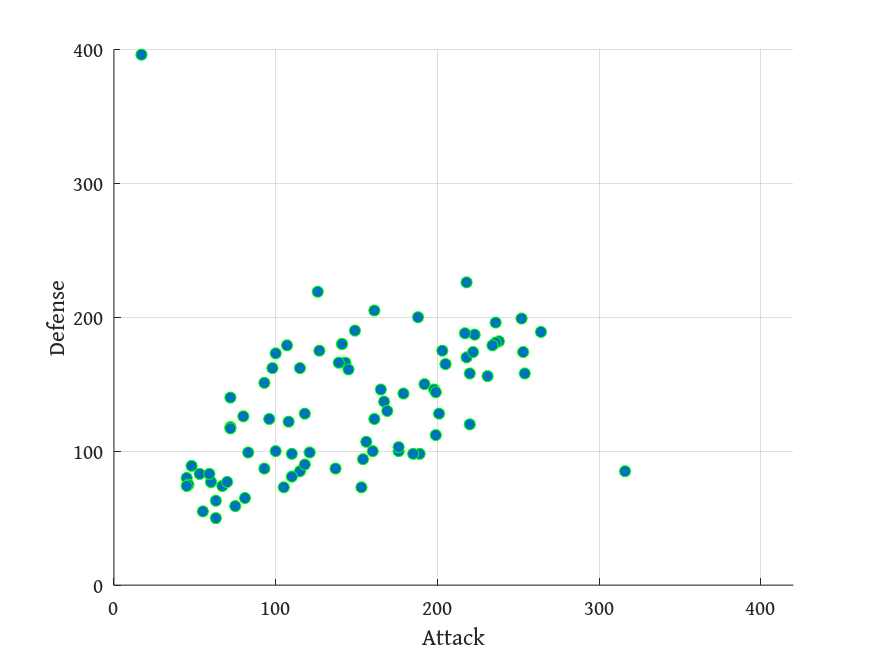
\includegraphics[width=.5\textwidth,keepaspectratio]{graph/BugDvA.png}
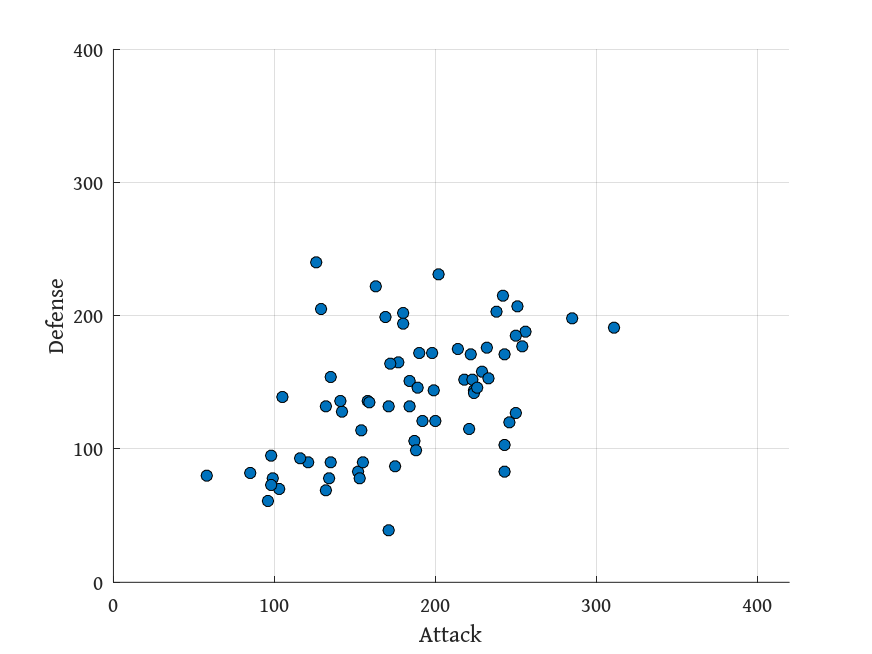
\includegraphics[width=.5\textwidth,keepaspectratio]{graph/DarkDvA.png}
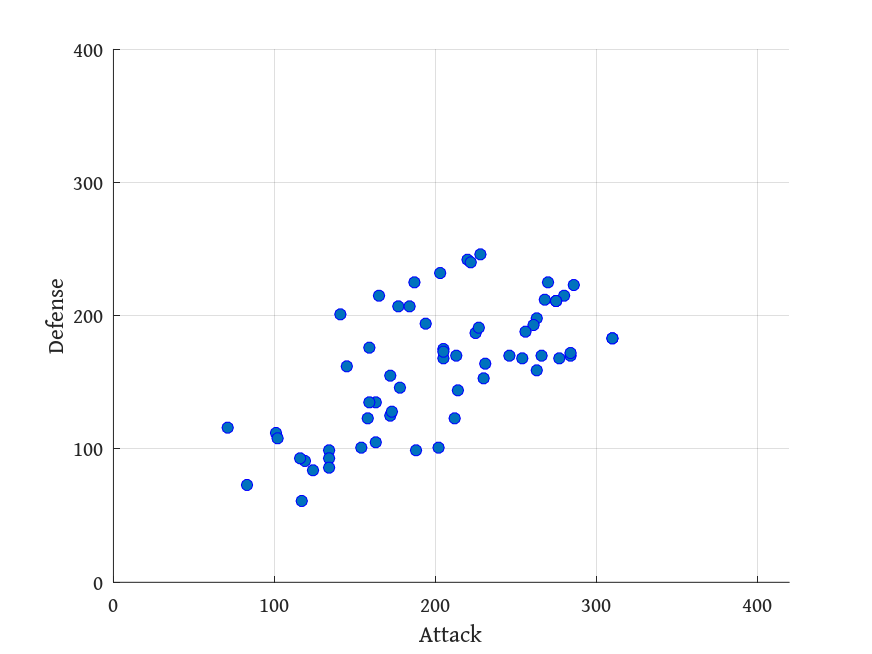
\includegraphics[width=.5\textwidth,keepaspectratio]{graph/DragonDvA.png}
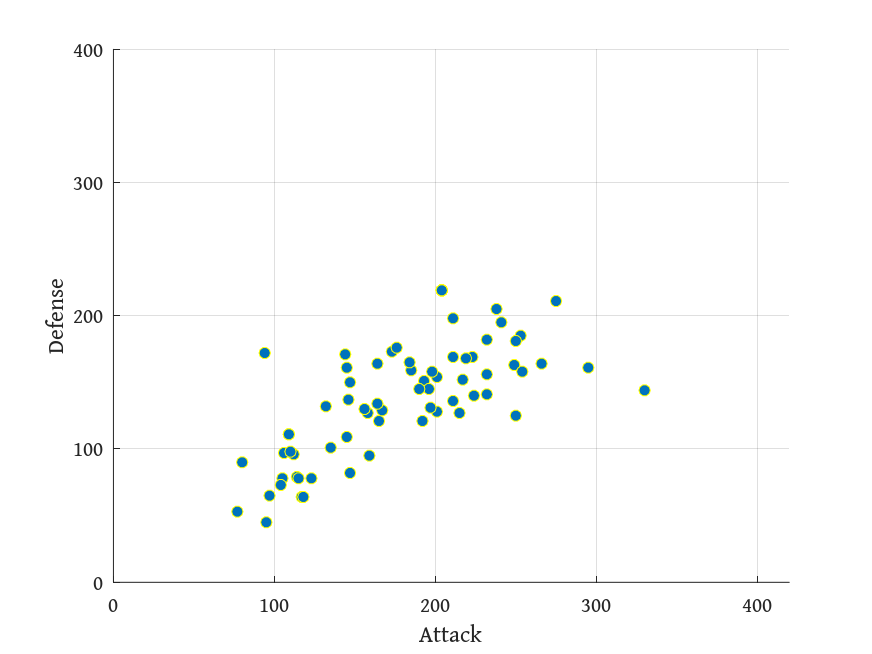
\includegraphics[width=.5\textwidth,keepaspectratio]{graph/ElectricDvA.png}
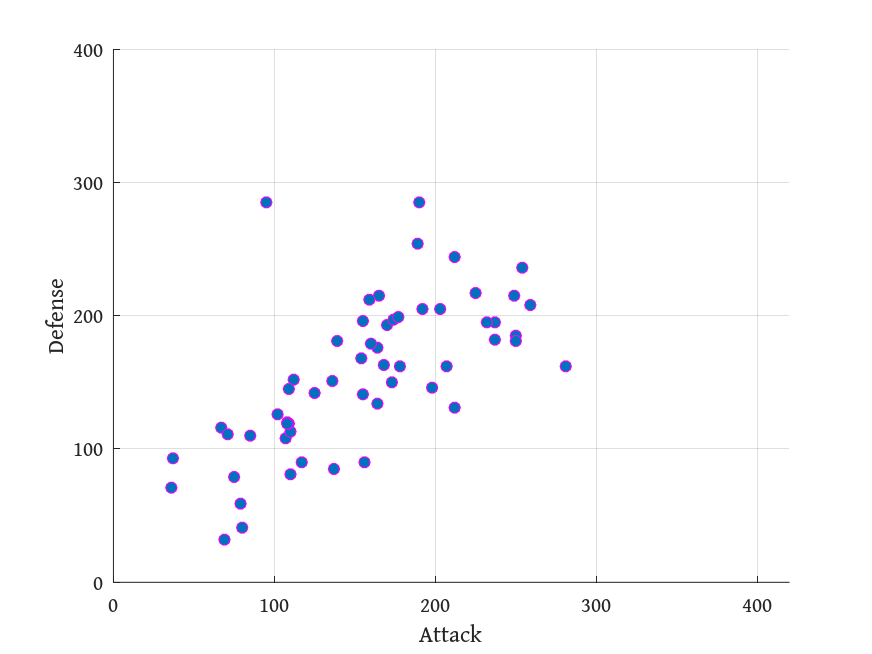
\includegraphics[width=.5\textwidth,keepaspectratio]{graph/FairyDvA.png}
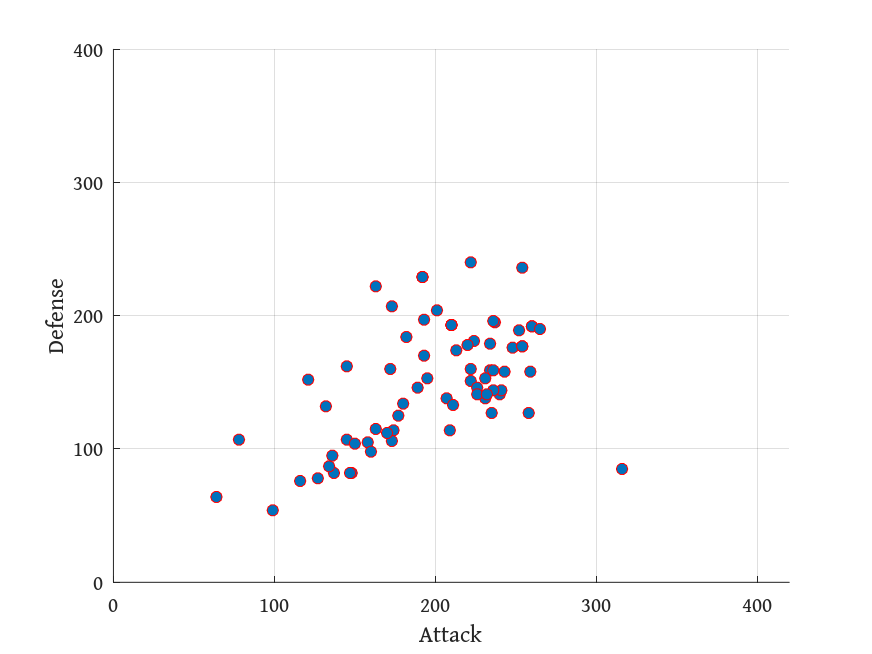
\includegraphics[width=.5\textwidth,keepaspectratio]{graph/FightingDvA.png}
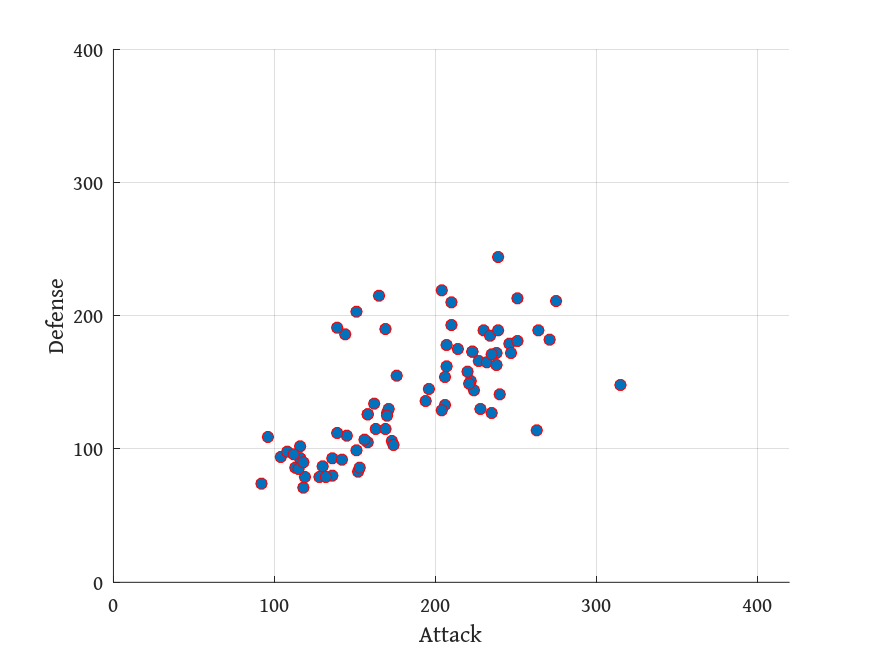
\includegraphics[width=.5\textwidth,keepaspectratio]{graph/FireDvA.png}
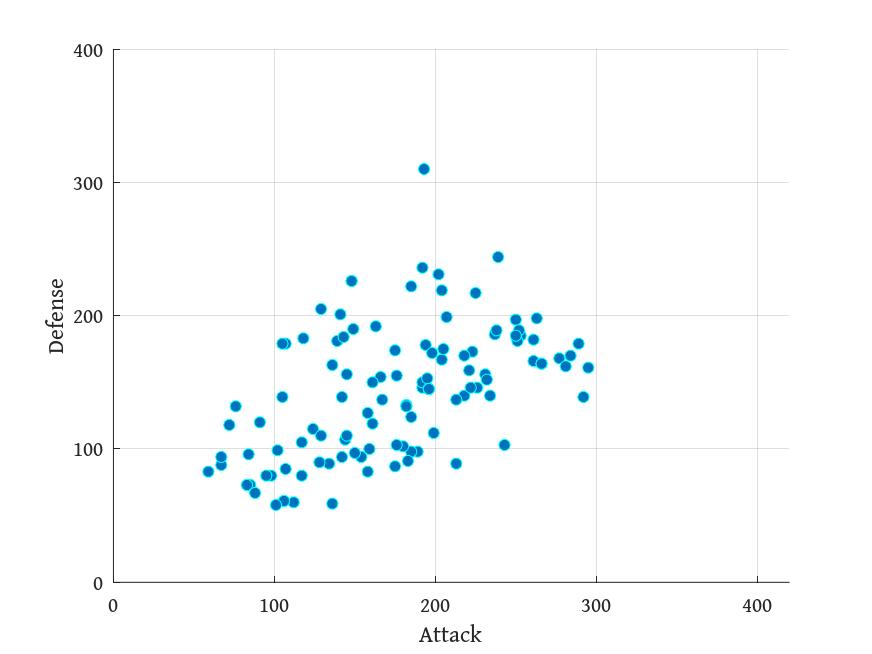
\includegraphics[width=.5\textwidth,keepaspectratio]{graph/FlyingDvA.png}
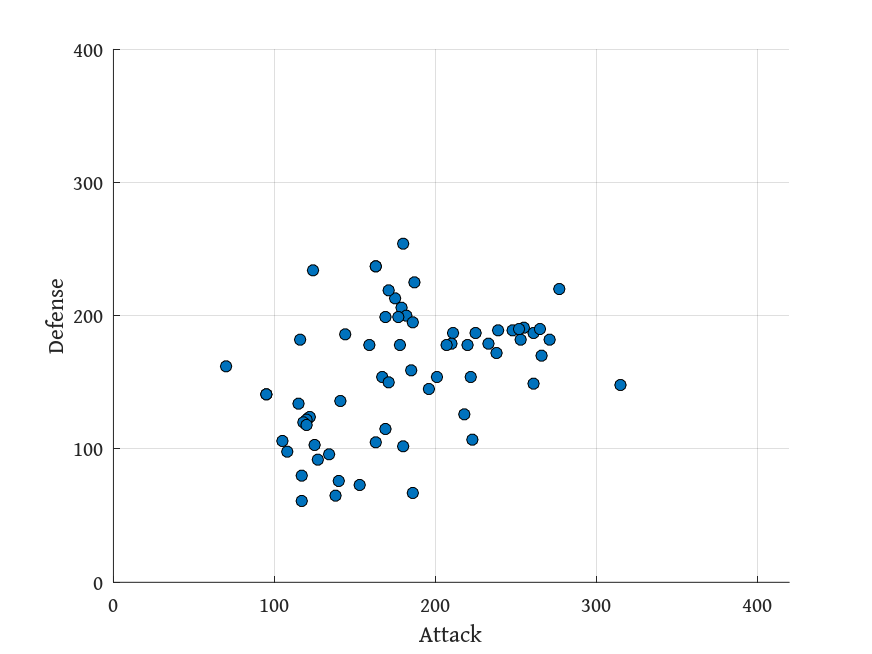
\includegraphics[width=.5\textwidth,keepaspectratio]{graph/GhostDvA.png}
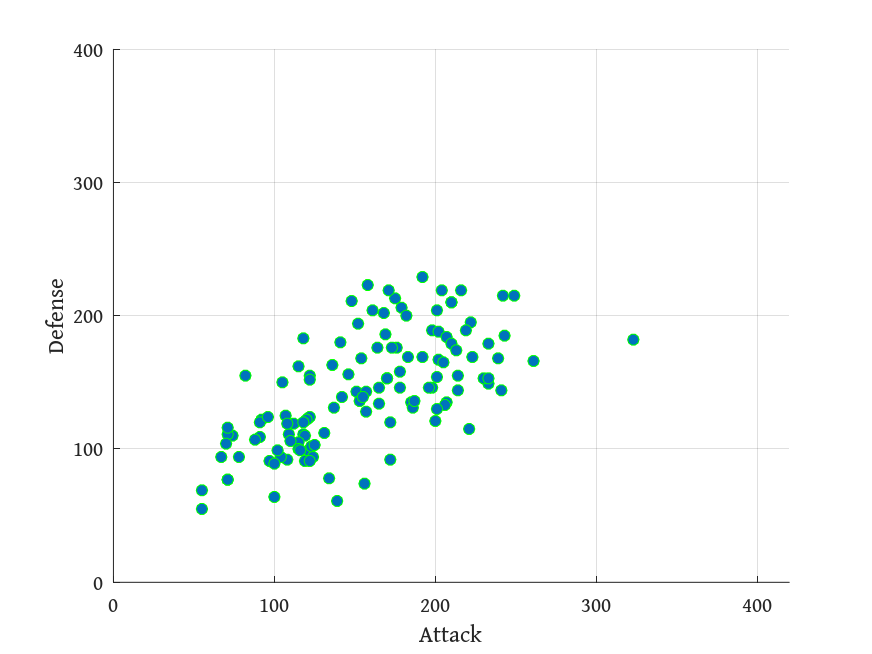
\includegraphics[width=.5\textwidth,keepaspectratio]{graph/GrassDvA.png}
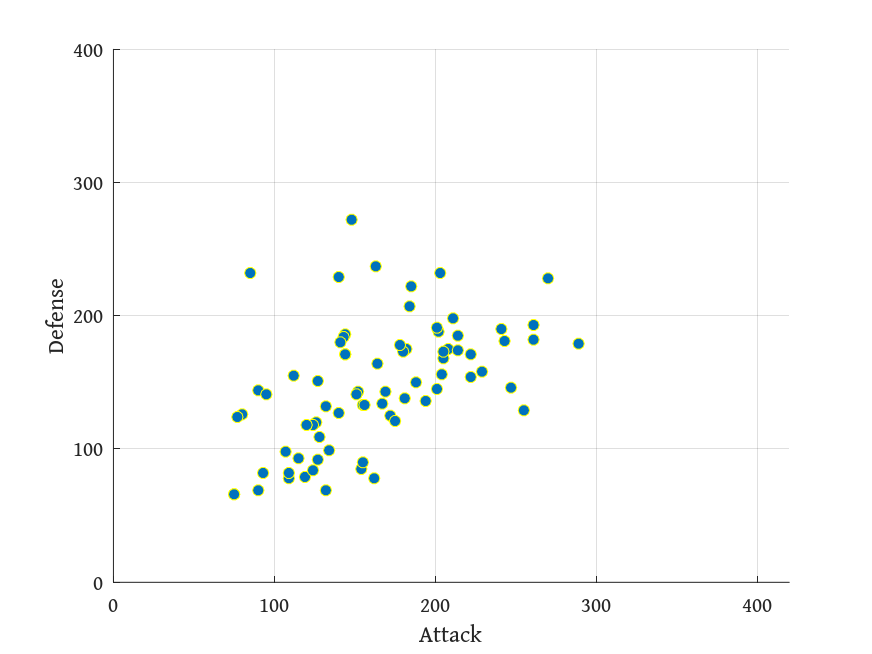
\includegraphics[width=.5\textwidth,keepaspectratio]{graph/GroundDvA.png}
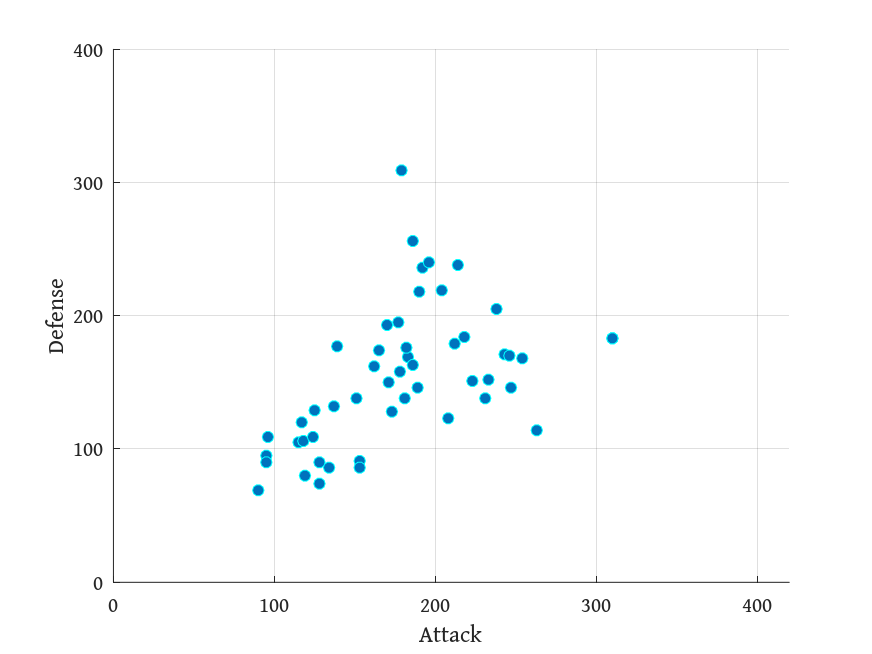
\includegraphics[width=.5\textwidth,keepaspectratio]{graph/IceDvA.png}
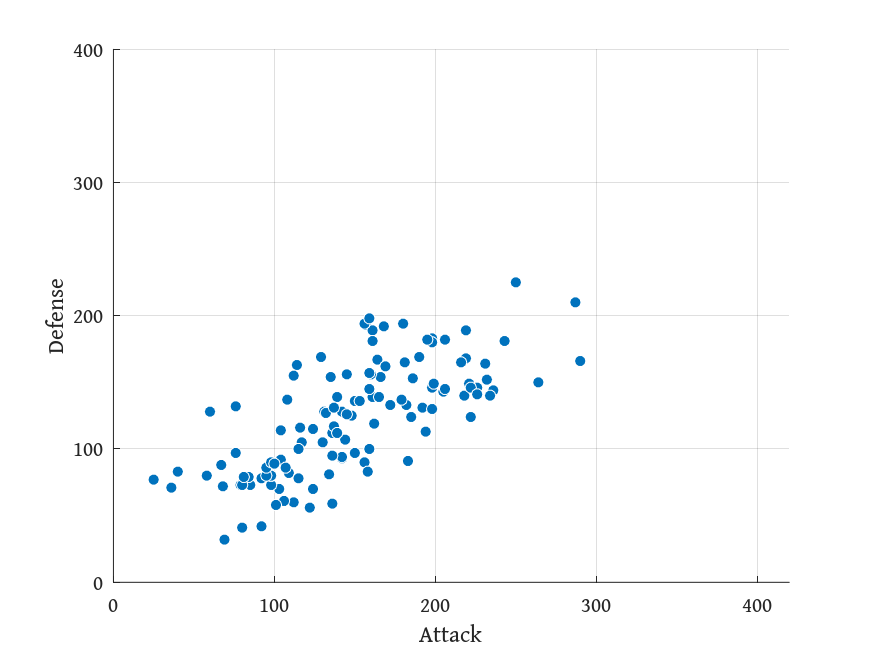
\includegraphics[width=.5\textwidth,keepaspectratio]{graph/NormalDvA.png}
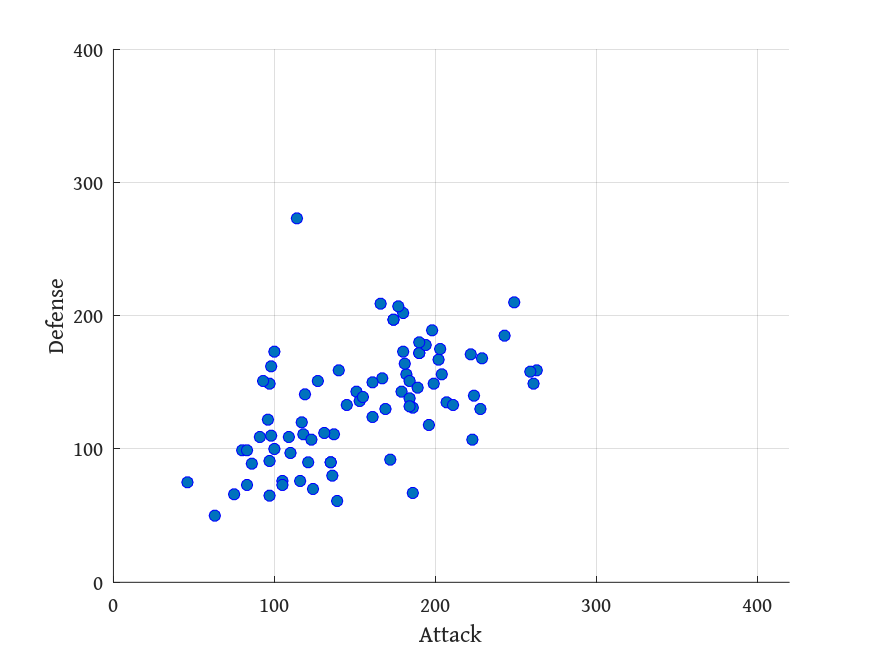
\includegraphics[width=.5\textwidth,keepaspectratio]{graph/PoisonDvA.png}
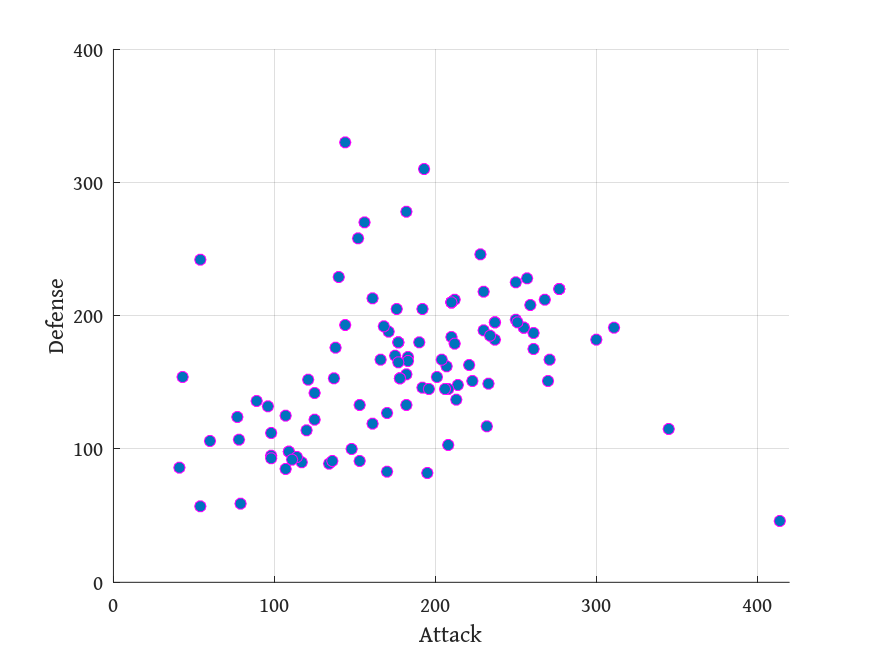
\includegraphics[width=.5\textwidth,keepaspectratio]{graph/PsychicDvA.png}
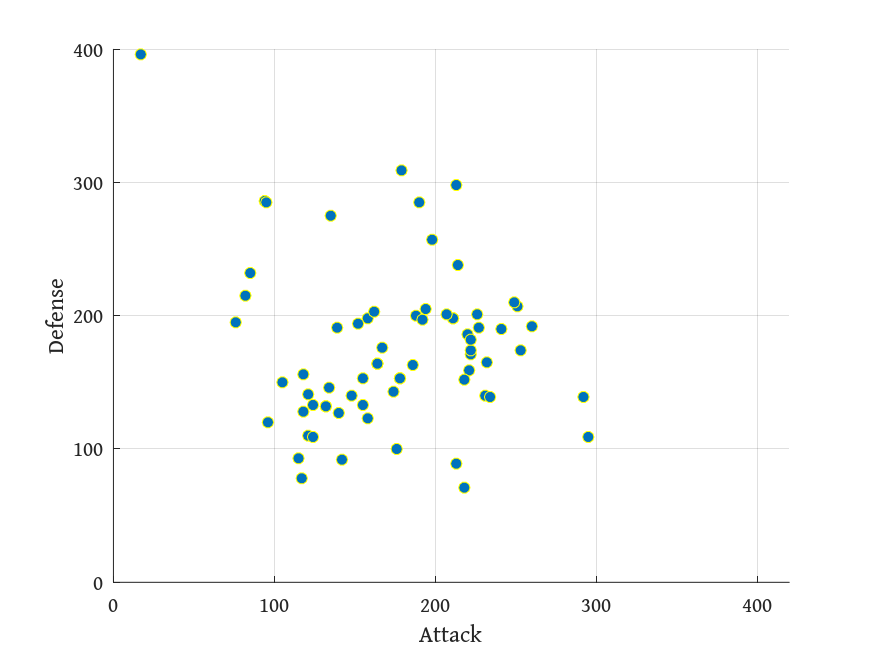
\includegraphics[width=.5\textwidth,keepaspectratio]{graph/RockDvA.png}
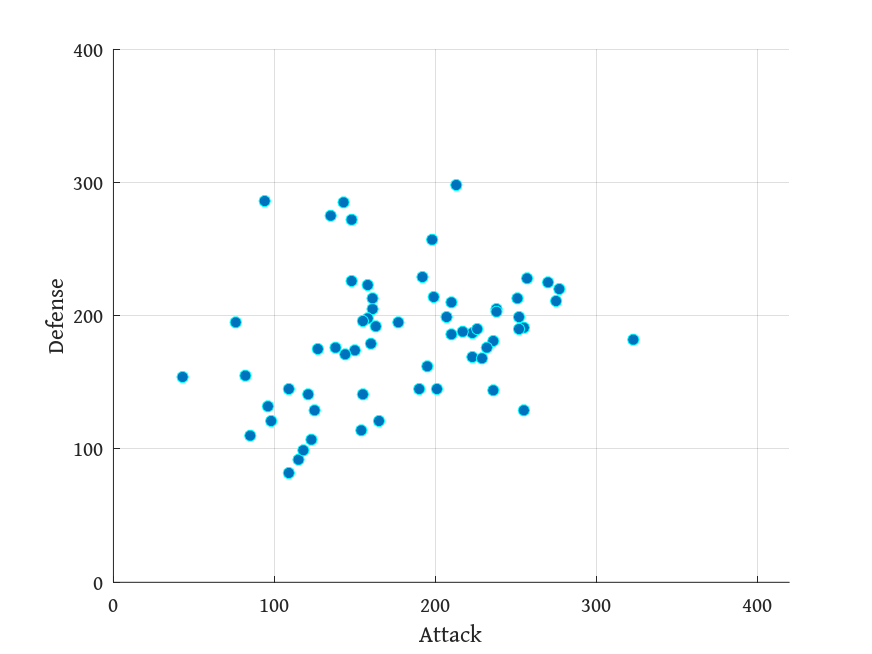
\includegraphics[width=.5\textwidth,keepaspectratio]{graph/SteelDvA.png}
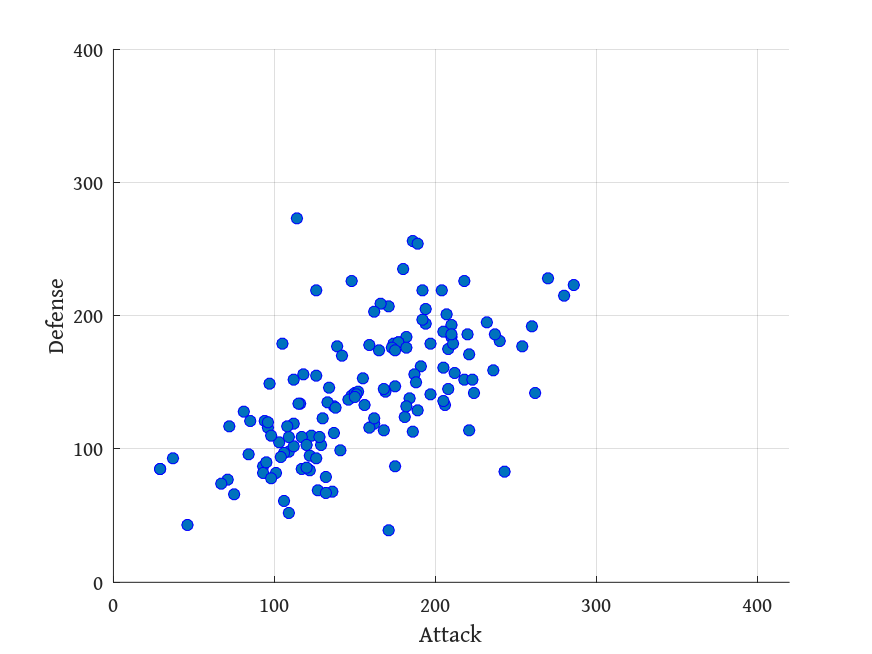
\includegraphics[width=.5\textwidth,keepaspectratio]{graph/WaterDvA.png}

\begin{figure}[h]
\centering
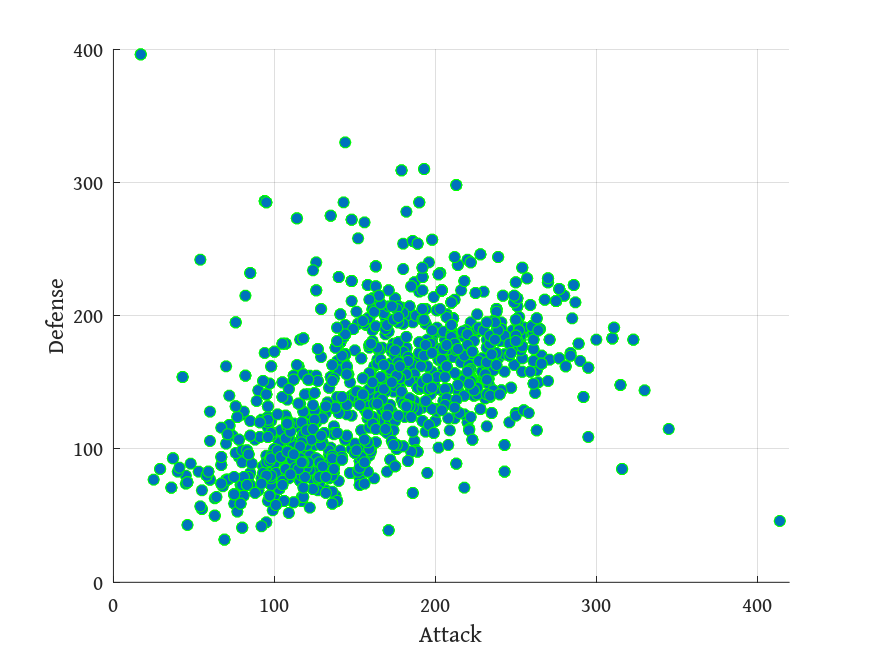
\includegraphics[width=\textwidth,keepaspectratio]{graph/AllDvA.png}
\caption{Defense vs Attack, all species}
\label{figure:alldva}
\end{figure}

Now we scatter stamina (max 500) against attack (max 420):

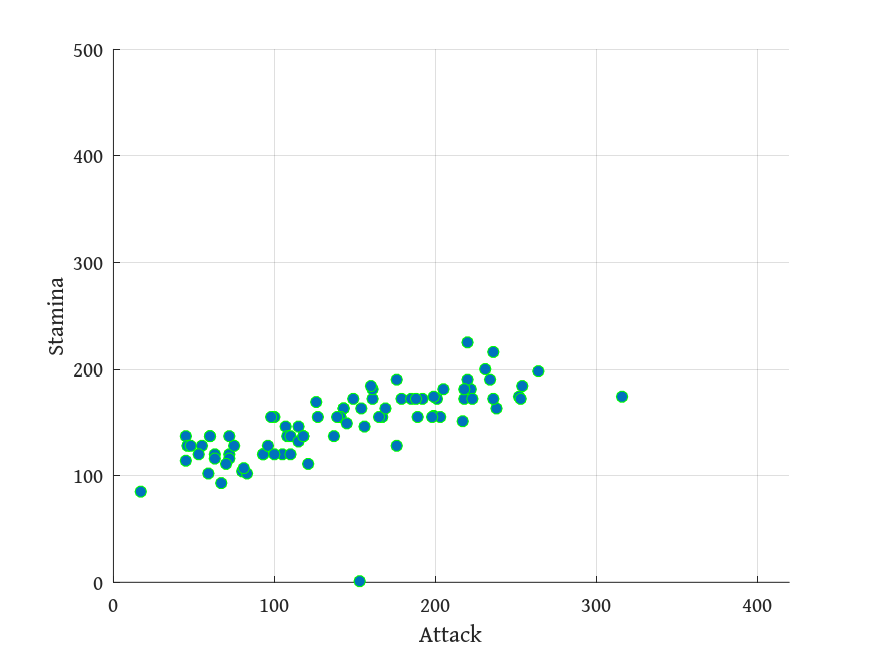
\includegraphics[width=.5\textwidth,keepaspectratio]{graph/BugSvA.png}
\includegraphics[width=.5\textwidth,keepaspectratio]{graph/DarkSvA.png}
\includegraphics[width=.5\textwidth,keepaspectratio]{graph/DragonSvA.png}
\includegraphics[width=.5\textwidth,keepaspectratio]{graph/ElectricSvA.png}
\includegraphics[width=.5\textwidth,keepaspectratio]{graph/FairySvA.png}
\includegraphics[width=.5\textwidth,keepaspectratio]{graph/FightingSvA.png}
\includegraphics[width=.5\textwidth,keepaspectratio]{graph/FireSvA.png}
\includegraphics[width=.5\textwidth,keepaspectratio]{graph/FlyingSvA.png}
\includegraphics[width=.5\textwidth,keepaspectratio]{graph/GhostSvA.png}
\includegraphics[width=.5\textwidth,keepaspectratio]{graph/GrassSvA.png}
\includegraphics[width=.5\textwidth,keepaspectratio]{graph/GroundSvA.png}
\includegraphics[width=.5\textwidth,keepaspectratio]{graph/IceSvA.png}
\includegraphics[width=.5\textwidth,keepaspectratio]{graph/NormalSvA.png}
\includegraphics[width=.5\textwidth,keepaspectratio]{graph/PoisonSvA.png}
\includegraphics[width=.5\textwidth,keepaspectratio]{graph/PsychicSvA.png}
\includegraphics[width=.5\textwidth,keepaspectratio]{graph/RockSvA.png}
\includegraphics[width=.5\textwidth,keepaspectratio]{graph/SteelSvA.png}
\includegraphics[width=.5\textwidth,keepaspectratio]{graph/WaterSvA.png}

\begin{figure}[hb]
\centering
\includegraphics[width=\textwidth,keepaspectratio]{graph/AllSvA.png}
\caption{Stamina vs Attack, all species}
\label{figure:alldva}
\end{figure}

\section{Freak Pokémon}
\label{sec:freaks}
A few Pokémon have unique behaviors or mechanics.

\subsection{Morpeko}
\label{subsec:morpeko}
Morpeko changes its form between ``Full Belly Mode'' and ``Hangry Mode''
  each time it uses a charged attack.
Upon becoming active, Morpeko is in Full Belly Mode, and Aura Wheel is an Electric attack.
In Hangry Mode, Aura Wheel is a Dark attack.
Morpeko cannot defend gyms, assault gyms, or participate in raids.

\subsection{Smeargle}
\label{subsec:smeargle}
Smeargle is not generally available in the wild\footnote{When captured in the wild, it knows Splash and Struggle.}.
Instead, it sometimes photobombs pictures taken of your Buddy Pokémon.
Smeargle will then spawn nearby, exclusive to the affected Trainer.
If caught, this Smeargle knows the same moves as whatever Pokémon was being photographed.
Smeargle will not appear more than once per day.

\subsection{Ditto}
\label{subsec:ditto}
At any time, there is a set of Pokémon which might actually be Ditto,
  a Pokémon impersonator (impokénator?).
When captured, the Pokémon will be revealed as Ditto, and Ditto Candy will take
  the place of expected Candy.
Ditto status is shared across Trainers, i.e. it is a property of the spawn, not the encounter.
In battle, Ditto adopts the moves, typing, ATK, and DEF of its opponent, but not its MHP\@.
The result is almost universally garbage, and Ditto can't be used in 3x3 anyway\footnote{It is one of two species banned from PvP, the other being Shedinja.}.

\subsection{Zygarde}
\label{subsec:zygarde}
Zygarde is received from research in its ``10\%'' form.
It can evolve to a ``50\%'' form, and a subsequent ``Complete'' form.
Zygarde Candy exists, but is not used for these evolutions.
Instead, ``Zygarde Cells'' are found on Routes, and can be stored in the Zygarde Cube
 (received at the same time as Zygarde 10\%).
The Cube can hold up to 300 cells, and cannot be removed from the bag.
Up to three cells can be collected per calendar day (more than three can spawn).
A route will not necessarily present a cell, cells are only generated the first
  time a route is taken each day, and more than one per route is very rare.
Cells usually show up near the end of a route.
If the route is marked complete, any spawned cells will disappear.
